\section{Character functions}
\begin{itemize}
    \item The cctype library includes very useful functions that allow us to work with characters, such as the following:
        \begin{itemize}
            \item Functions for testing characters.
            \item Functions for converting character case.
        \end{itemize}
    \item In order to use those functions you must include the library.
        \begin{minted}[autogobble]{cpp}
            #include <cctype>
        \end{minted}
    
    \item The testing functions accept a single character and all evaluate to a boolean value, the conversion functions return the converted character.
    \item Some of the testing functions are:
        \begin{itemize}
            \item To use them you must pass the character to evaluate.
        \end{itemize}
        \begin{center}
            \begin{tabular}{ |c|c| }
                \hline 
                    \mintinline{cpp}{isalpha(c)} & True if c is a letter. \\
                    \mintinline{cpp}{isalnum(c)} & True if c is a letter or digit. \\
                    \mintinline{cpp}{isdigit(c)} & True if c is a digit. \\
                    \mintinline{cpp}{islower(c)} & True if c is lowercase letter. \\
                    \mintinline{cpp}{isprint(c)} & True if c is a printable character. \\
                    \mintinline{cpp}{ispunct(c)} & True if c is a punctuation character. \\
                    \mintinline{cpp}{isupper(c)} & True if c is an uppercase letter. \\
                    \mintinline{cpp}{isspace(c)} & True if c is whitespace. \\
                \hline
            \end{tabular}
        \end{center}
    
    \item Character conversion functions:
        \begin{center}
            \begin{tabular}{ |c|c| }
                \hline
                    \mintinline{cpp}{tolower(c)} & returns lowercase of c, if the function can't convert, it will return to the character that was passed in. \\
                    \mintinline{cpp}{toupper(c)} & returns uppercase of c, if the function can't convert, it will return to the character that was passed in. \\
                \hline
            \end{tabular}
        \end{center}
\end{itemize}


%----------------------------------------------------------------------------------------
\section{C-Style strings}
\begin{itemize}
    \item A C-Style string is a sequence of characters:
        \begin{itemize}
            \item Stored contiguous in memory.
            \item Implemented as an array of characters. You can access each character using the array subscript syntax.
            \item Terminated by a null character (null).
                \begin{itemize}
                    \item Null character with a value of zero.
                \end{itemize}
            \item Refered to as zero or null terminated strings.
        \end{itemize}
    
    \item String literal:
        \begin{itemize}
            \item Sequence of characters in double quotes.
            \item Constant.
            \item Terminated with a null character.
        \end{itemize}
    
    \item How C++ stores strings in memory:
        \begin{figure}[H]
            \centering
            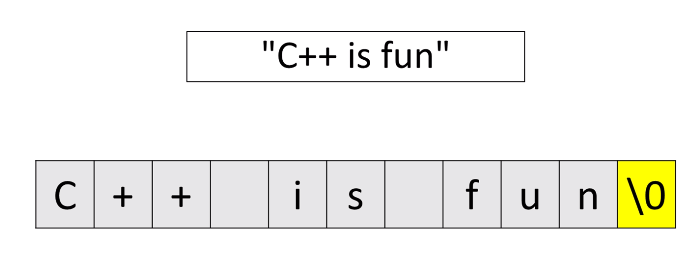
\includegraphics[width=0.4\textwidth]{./figs/stringmem}
            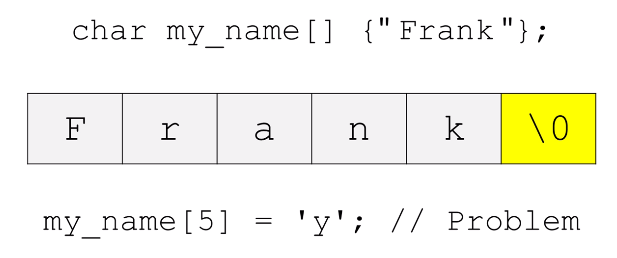
\includegraphics[width=0.4\textwidth]{./figs/stringmem1}
            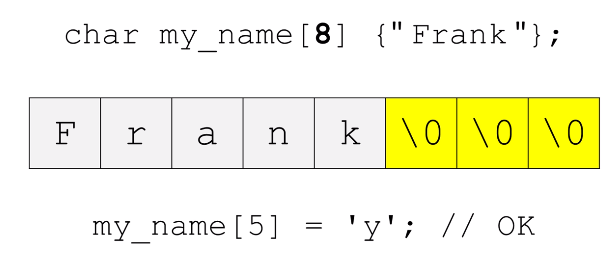
\includegraphics[width=0.4\textwidth]{./figs/stringmem2}
            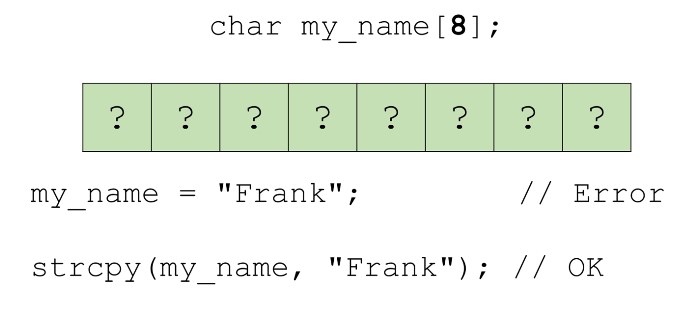
\includegraphics[width=0.4\textwidth]{./figs/stringmem3}
        \end{figure}
    
    \item The cstring library contains functions that work with C-style strings, these serve for: (include the library \mintinline{cpp}{#include <cstring>})
        \begin{itemize}
            \item Copying.
            \item Concatenation.
            \item Comparison.
            \item Searching.
            \item And others.
        \end{itemize}
    
    \item C++ has a library called cstdlib, containing functions that convert C-Style strings to other types, such as:
        \begin{itemize}
            \item Integer.
            \item Float.
            \item Long.
            \item Etc.
        \end{itemize}
\end{itemize}

\subsection{Examples}
\begin{itemize}
    \item Example of string functions:
        \begin{minted}[autogobble]{cpp}
            #include <iostream>
            #include <cstring>
            using namespace std;
            int main() {
                char str[80];
                strcpy(str, "Hello "); // copy.
                strcat(str, "there "); // concatenate.
                cout << strlen(str); // 10
                strcmp(str, "Another"); // -1
                return 0;
            }
            /* OUTPUT:
            12
            */
        \end{minted}
\end{itemize}


%----------------------------------------------------------------------------------------
\section{Working with C-Style strings examples}
\begin{itemize}
    \item Example:
        \begin{minted}[autogobble]{cpp}
            #include <iostream>
            #include <cstring>
            using namespace std;
            int main() {
                char first_name[20] {};
                char last_name[20] {};
                char full_name[20] {};
                char temp[50] {};
                cout << "Please enter your first and last name: ";
                cin >> first_name >> last_name;
                cout << "--------------------------" << endl;
                cout << "Hello, " << first_name << " your first name has " << strlen(first_name) << " characters." << endl;

                strcpy(full_name, first_name);
                strcat(full_name, " ");
                strcat(full_name, last_name);

                cout << full_name << endl; 
                return 0;
            }
            /* OUTPUT:
            Please enter your first and last name: David Corzo
            --------------------------
            Hello, David your first name has 5 characters.
            David Corzo

            */
        \end{minted}
    
    \item In the last example we read in the firs name and the last name separately, the program delimited the space entered by the user. In this example we will read in the full name with the space.
        \begin{minted}[autogobble]{cpp}
            #include <iostream>
            #include <cstring>
            using namespace std;
            int main() {
                char full_name[50] {};
                cout << "Please enter your first and last name: ";
                cin.getline(full_name, 50); // it will stop at 50 chars or when it finds the return character.
                cout << full_name << endl;
                return 0;
            }
            /* OUTPUT:
            Please enter your first and last name: David Corzo
            David Corzo

            */
        \end{minted}
    
    \item Comparing strings:
        \begin{minted}[autogobble]{cpp}
            #include <iostream>
            #include <cstring>
            using namespace std;
            int main() {
                char str1[] {"Hello world\n"};
                char str2[] {"Hello world\n"};
                if (strcmp(str1, str2) == 0) {
                    cout << "The strings are the same." << endl;
                }
                return 0;
            }
            /* OUTPUT:
            The strings are the same.

            */
        \end{minted}
    
    \item Iterating and changing strings:
        \begin{minted}[autogobble]{cpp}
            #include <iostream>
            #include <cstring>
            using namespace std;
            int main() {
                char str1[] {"Hello world."};
                for (size_t i {0}; i < strlen(str1); ++i) {
                    if (isalpha(str1[i])) {
                        str1[i] = toupper(str1[i]);
                    }
                }
                cout << str1 << endl;
                return 0;
            }
            /* OUTPUT:
            HELLO WORLD.

            */
        \end{minted}
\end{itemize}


%----------------------------------------------------------------------------------------
\section{C++ strings}
\begin{itemize}
    \item \mintinline{cpp}{std::string} is a class in the C++ Standard template library.
        \begin{itemize}
            \item You must include the library \mintinline{cpp}{#include <string>}.
            \item You must include the \mintinline{cpp}{std} namespace.
            \item Stored contiguous in memory.
            \item Dynamic size.
            \item Work with input and output streams.
            \item There are lots of useful member functions.
            \item Our familiar operators can be used (\mintinline{cpp}{+,=,<,<=,>,>=,+=,==,!=,[],}...). They also work with the insertion and extraction operator. This is another example of operator overloading.
            \item Can be converted to C-Style strings if needed.
            \item Safer to use.
        \end{itemize}
    
    \item Declaring and initializing:
        \begin{itemize}
            \item You can initialize a C++ string using any initialization style. 
            \item C++ strings are always initialized, unlike C-style strings that were never initialized.
        \end{itemize}
        \begin{minted}[autogobble]{cpp}
            #include <iostream>
            #include <string>
            using namespace std;
            int main() {
                string s1; // Empty.
                string s2 {"Frank"}; // Frank
                string s3 {s2}; // Frank
                string s4 {"Frank", 3}; // Fra
                string s5 {s3,0,2}; // Fr
                string s6 (3, 'X'); // XXX
                return 0;
            }
        \end{minted}
    
    \item With C++ strings you can use the assignment operator.
        \begin{minted}[autogobble]{cpp}
            #include <iostream>
            #include <string>
            using namespace std;
            int main() {
                string s1;
                s1 = "C++";
                string s2;
                s2 = s1;
                return 0;
            }
        \end{minted}
    
    \item Concatenation can be done with the \mintinline{cpp}{+} operator.
        \begin{itemize}
            \item In the below example if we would have tried to do something as:
                \begin{minted}[autogobble]{cpp}
                    sentence = "C++" + " is powerful";
                \end{minted}
            \item We would have had a compiler error, because as far as C++ is concerned these are two C-Style literals, not \mintinline{cpp}{std::string} objects, thus addition is not concatenation.
            \item A combination of C-style strings and C++ strings is ok, the code below does this, however you cannot add two C-Style strings.
        \end{itemize}
        \begin{minted}[autogobble]{cpp}
            #include <iostream>
            using namespace std;
            int main() {
                string part1 {"C++"};
                string part2 {"is powerful"};
                string sentence;
                sentence = part1 + " " + part2 + " language";
                cout << sentence << endl;
                return 0;
            }
            /* OUTPUT:
            C++ is powerful language
            */
        \end{minted}
    
    \item Accessing characters [] and at() method:
        \begin{itemize}
            \item The difference between the [] and the .at() method is that the .at() method in the \mintinline{cpp}{std::string} performs bounds checking and the [] does not. As a best practice, always use the .at() method.
        \end{itemize}
        \begin{minted}[autogobble]{cpp}
            #include <iostream>
            using namespace std;
            int main() {
                string s1;
                string s2 {"Frank"};
                cout << s2[0] << endl; // F
                cout << s2.at(0) << endl; // F
                return 0;
            }
            /* OUTPUT:
            F
            F

            */
        \end{minted}
        \begin{minted}[autogobble]{cpp}
            #include <iostream>
            #include <string>
            using namespace std;
            int main() {
                string s1 {"Frank"};
                for (char c : s1) {
                    cout << c << endl;
                }
                return 0;
            }
            /* OUTPUT:
            F
            r
            a
            n
            k

            */
        \end{minted}
    
    \item Comparing \mintinline{cpp}{std::string} objects can be done with the \mintinline{cpp}{==, !=, >, >=, <, <=} operators. We can perform comparisons in the following cases: 
        \begin{itemize}
            \item When we have two \mintinline{cpp}{std::string} objects.
            \item When we have one \mintinline{cpp}{std::string} object and C-style string literal.
            \item When we have \mintinline{cpp}{std::string} object and C-style string variable.
            \item We cannot perform this comparison if both are string literals.
            \item Greater than, less than, or equal are done by comparing the values in the ASCII table.
        \end{itemize}
        \begin{minted}[autogobble]{cpp}
            #include <iostream>
            #include <string>
            using namespace std;
            int main() {
                cout << boolalpha;
                string s1 {"Apple"};
                string s2 {"Banana"};
                string s3 {"Kiwi"};
                string s4 {"apple"};
                string s5 {s1};
                cout << (s1 == s5) << endl; // true
                cout << (s1 == s2) << endl; // false
                cout << (s1 != s2) << endl; // true
                cout << (s2 > s1) << endl; // true
                cout << (s4 < s5) << endl; // false
                cout << (s1 == "Apple") << endl; // true
                return 0;
            }
            /* OUTPUT:
            true
            false
            true
            true
            false
            true

            */
        \end{minted}
    
    \item You can extract substrings from a string using the \mintinline{cpp}{substr()} method.
        \begin{itemize}
            \item This method extracts a substring from a \mintinline{cpp}{std::string}.
                \begin{minted}[autogobble]{cpp}
                    object.substr(start_index, lenght);
                \end{minted}
        \end{itemize}
        \begin{minted}[autogobble]{cpp}
            #include <iostream>
            #include <string>
            using namespace std;
            int main() {
                string s1 {"This is a test"};
                cout << s1.substr(0,4) << endl; // This
                cout << s1.substr(5,2) << endl; // is
                cout << s1.substr(10,4) << endl; // test
                return 0;
            }
            /* OUTPUT:
            This
            is
            test

            */
        \end{minted}
    
    \item To find a substring in a \mintinline{cpp}{std::string} you can use the \mintinline{cpp}{find()} method.
        \begin{itemize}
            \item This method returns the index of a substring in a \mintinline{cpp}{std::string}.
                \begin{minted}[autogobble]{cpp}
                    object.find(search_string);
                \end{minted}
        \end{itemize}
        \begin{minted}[autogobble]{cpp}
            #include <iostream>
            #include <string>
            using namespace std;
            int main() {
                string s1 {"This is a test"};
                cout << s1.find("This") << endl;
                cout << s1.find("This") << endl;
                cout << s1.find("is") << endl;
                cout << s1.find("test") << endl;
                cout << s1.find('e') << endl;
                cout << s1.find("is",4) << endl; // The 4 represents from what index forward you want to start to look.
                cout << s1.find("XX") << endl; // its not found so the value returned is string::npos
                return 0;
            }
            /* OUTPUT:
            0
            0
            2
            10
            11
            5
            18446744073709551615

            */
        \end{minted}
        \begin{itemize}
            \item There is also an \mintinline{cpp}{.rfind} method that starts searching from the end of the string.
        \end{itemize}
    
    \item You can also remove characters using the \mintinline{cpp}{erase()} and \mintinline{cpp}{clear()} methods.
        \begin{itemize}
            \item This methods removes a substring of characters from a \mintinline{cpp}{std::string}.
                \begin{minted}[autogobble]{cpp}
                    object.erase(start_index, lenght);
                \end{minted}
        \end{itemize}
        \begin{minted}[autogobble]{cpp}
            #include <iostream>
            #include <string>
            using namespace std;
            int main() {
                string s1 {"This is a test"};
                cout << s1.erase(0,5) << endl;
                cout << s1.erase(5,4) << endl;
                s1.clear(); // clears the string.
                return 0;
            }
            /* OUTPUT:
            is a test
            is a

            */
        \end{minted}
    
    \item To obtain the length of the string use:
        \begin{minted}[autogobble]{cpp}
            object.length();
        \end{minted}
    
    \item To cocatenate you can use the \mintinline{cpp}{+=} operator:
        \begin{minted}[autogobble]{cpp}
            s1 += " James"; // concatenates s1 and " James".
        \end{minted}

    
    \item Input with C++ strings:
        \begin{itemize}
            \item The \mintinline{cpp}{cin} reads until it finds a space, sometimes we want to read up until the user enters the return character. For this we can use \mintinline{cpp}{getline(cin, s1);}.
        \end{itemize}
        \begin{minted}[autogobble]{cpp}
            #include <iostream>
            #include <string>
            using namespace std;
            int main() {
                string s1;

                getline(cin, s1); // reads entire line.
                cout << s1 << endl;

                getline(cin, s1, 'x'); // you can add a delimeter.
                cout << s1 << endl;
                return 0;
            }
            /* OUTPUT:
            Hello world
            Hello world
            Hello world x
            Hello world

            */
        \end{minted}
\end{itemize}
